\documentclass[12pt,letterpaper,twoside]{book}
\usepackage[utf8]{inputenc}
\usepackage[spanish]{babel}
\usepackage{amsmath}
\usepackage{amsfonts}
\usepackage{amssymb}
\usepackage{makeidx}
\usepackage{graphicx}
\usepackage{lmodern}
\usepackage{kpfonts}
\usepackage[left=2cm,right=2cm,top=2cm,bottom=2cm]{geometry}


\title{Descripción general del Controlador de Lógica Difusa Para un Biodigestor Anaeróbico}
\author{Dr. Casimiro Gómez González\\
	Facultad de Electrónica, UPAEP\\
               correo: casimiro.gomez@upaep.mx\\
               Tel: 222 229 9428}
\date{Primavera 2013}
\begin{document}
\frontmatter
\maketitle


\chapter{Prólogo}
El presente material ha sido desarrollado como parte del proyecto de investigación, financiado por la secretaria de energía de México y el Consejo Nacional de Ciencia y Tecnología de México (CONACYT) y es un resumen de controlador que se esta desarrollando en el Laboratorio de Sistemas Embebidos (LSE) de la Universidad Popular Autónoma del Estado de Puebla (UPAEP) en México.
\begin{flushright}

El autor\\
Casimiro Gómez González\\
Doctor en Ingeniería Mecatrónica
\end{flushright}

%\tableofcontents
%\listoftables
%\listoffigures

\mainmatter
\chapter{El sistema de control}

El sistema de control esta compuesto por tres subsistemas:
\begin{itemize}
\item El controlador FACS
\item El sistema preditor de Lógica Difusa
\item El administrador de Energía basado en lógica difusa
\end{itemize}
En la figura \ref{fig001} se muestra la relación de el controlador FACTS (Flexible AC Transmission System) en todo el sistema. La función principal del controlador FACTS es estimar la inyecciones de corriente para corregir en tiempo real los flujos de energía que provienen del motogenerador y del sistema fotovoltaico, con la intensión de mantener un suministro constante de energía a la red del usuario, a través de un tablero de transferencia controlado por unos controladores de corriente.

El controlador FACTS recibe como señales de entrada:

\begin{itemize}
\item La señal en tiempo real del voltaje y la corriente del motogenerador
\item La señal en tiempo real del voltaje y la corriente del Sistema Fotovoltaico
\end{itemize}

Con estas dos señales el controlador envía:

\begin{itemize}
\item La señal a los controladores de corriente para inyectar mas o menos corriente del motogenerador
\item La señal a los controladores de corriente para inyectar mas o menos corriente del sistema Fotovoltaico
\end{itemize}

\section{El sistema Predictor de Lógica Difusa}

En la figura \ref{fig002} se muestra el diagrama de señales principales para el controlador de lógica difusa para el biodigestor. En el se muestran las principales señales de entrada y de salida del controlador, entendiendo como señales de entrada y salida a aquellas que varían con el tiempo para un proceso determinado. 

\begin{figure}
\centering
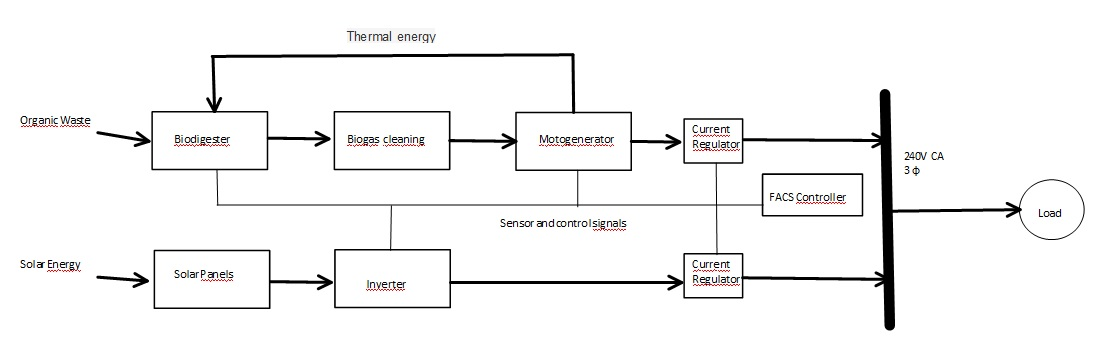
\includegraphics[width=6.5in]{GeneraldeEnergia.jpg}
\caption{Diagrama de señales del controlador de Lógica Difusa Subsistema Biodigestor}
\label{fig001}
\end{figure}

La descripción de las señales es la siguiente:
\begin{itemize}
\item $S_{entrada}$ es la concentración de entrada (en gDQO/L)
\item $Q_{entrada}$ es la velocidad del flujo de entrada (en L/h)
\item $Q_{gas-medido}$ es la velocidad del flujo de salida del biogas medido, incluyendo $CH_4$, $CO_2$, entre otros
\item $Q_{gas-calculado}$ es la velocidad del flujo de salida del biogas calculado, incluyendo $CH_4$, $CO_2$, entre otros
\item $pH$ y $T$ son las mediciones de los sensores de temperatura y pH
\end{itemize}

\begin{figure}
\centering
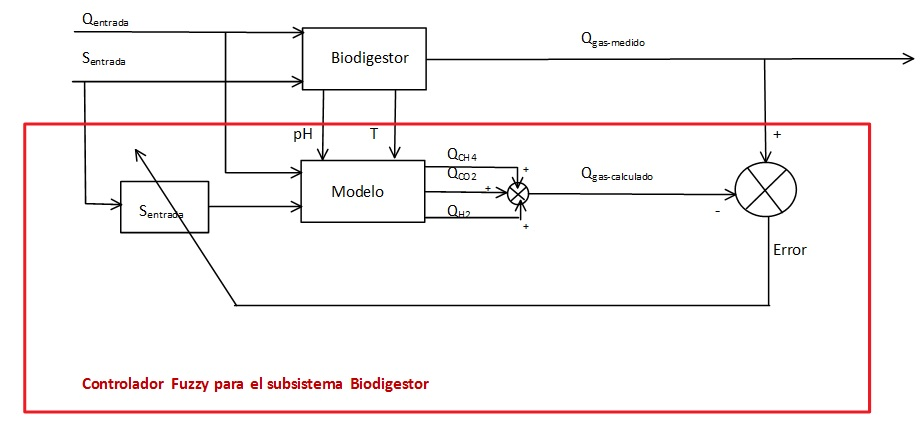
\includegraphics[width=6.5in]{controladorBio.jpg}
\caption{Controlador para el subsistema Biodigestor}
\label{fig002}
\end{figure}

\section{Parámetros}


La estimación de parámetros para las variables de lógica difusa y la técnica que se utiliza para ajustarlos son fundamental para la óptima predicción del comportamiento del biodigestor. Los mecanismos incluidos para describir los procesos fisico químicos y las reacciones de ácido base pueden llegar a ser sumamente complejos, solo en el modelo ADM1 se utilizan 32 variables de estado dinámicas de concentración y 6 procesos cinéticos ácido-base por contenedor. Si se considera el conjunto de ecuaciones diferencial y algebraica (DAE), hay 26 variables de estado dinámicas de concentración, 19 de procesos bioquímicos cinéticos, entre otros. Sin embargo, estos modelos determinísticos pueden ser simplificados para un proceso determinado por medio de estimación de parámetros utilizando técnicas de ajustes, en la literatura es posible utilizar desde modelos muy simplificados de estimación hasta modelos basados en resultados teóricos tomados de base de datos. Actualmente en nuestro proyecto se están tomando en consideración tres fuentes principales para estimar estos parámetros: 1.- El primero, es la literatura de la cual se ha tomado como base para el diagrama mostrado en la figura \ref{fig002}, 2.- Es las regresiones realizadas sobre los datos medidos para obtener ecuaciones de comportamiento del sistema y el estudio subsecuente de predecir en base a los parámetros estimados, y 3.- La modificación del modelo ADM1.

Como es obvio hay parámetros que pueden ser medidos de manera directa y otros que deben ser estimados de manera indirecta en el sistema. Debido al alto costo que representa su monitoreo en tiempo real.

\section{Conclusión}
Se ha descrito de manera muy general las variables de entrada y salida del controlador. La estimación de parámetros es la etapa en la cual se esta trabajando actualmente en el proyecto. Cualquier sugerencia o comentario quedamos a sus ordenes.

\bibliographystyle{alpha} %% plain.bst
\bibliography{./BiodigestorBibliografia}
\backmatter
\end{document}

